\section{Model Selection}
\label{sec:model-selection}

\subsection{K-fold Cross Validation}
\label{sec:model-selection:k-fold}

I use K-fold cross-validation to perform model selection.
The training set is randomly divided into K sub-sets.
Given a model $f$, we train the model with removing $k^{\mathrm{th}}$ fold data, and use the $k^{\mathrm{th}}$ fold data to test the model:
\begin{eqnarray}
    CV\left(\hat{f}\right) & = & \dfrac{1}{N}\sum_{i=1}^{N} L\left(y_i,\hat{f}^-k\left(x_i\right)\right)
    \label{eqn:cv}
\end{eqnarray}

\subsection{Akaike information criterion (AIC)}
\label{sec:model-selection:aic}

The second model selection method is the Akaike information criterion (AIC).
The AIC equation is:
\begin{eqnarray}
    AIC\left(\alpha\right) & = & \overline{err}\left(\alpha\right) + 2 \dfrac{d\left(\alpha\right)}{N}
    \hat{\sigma}_\varepsilon^2
\end{eqnarray}
where $\overline{err}\left(\alpha\right)$ is the training error, and $d\left(\alpha\right)$ is the number of parameters.

\subsection{Results}
\label{sec:model-selection:results}
\begin{table}
    \centering
    \caption{Models}
    \label{tab:models}
    \begin{tabular}{c|c}
        \hline\hline
        Model & Description \\\hline\hline
        Reduced Rank LDA & LDA model; Reduce dimension with Reduced Rank LDA ($N=19$) \\
        PCA + LDA & LDA model; Reduce dimension with PCA ($N=112$) \\
        PCA + SVM-1 & SVM model with linear kernel; Reduce dimension with PCA ($N=112$) \\
        PCA + SVM-2 & SVM model with kernel $p=2$; Reduce dimension with PCA ($N=112$) \\
        PCA + SVM-3 & SVM model with kernel $p=3$; Reduce dimension with PCA ($N=112$) \\
        PCA + MLP-100 & MLP model with 100 hidden neurons; Reduce dimension with PCA ($N=112$) \\
        PCA + MLP-200 & MLP model with 200 hidden neurons; Reduce dimension with PCA ($N=112$) \\
        PCA + MLP-300 & MLP model with 300 hidden neurons; Reduce dimension with PCA ($N=112$) \\
        PCA + MLP-400 & MLP model with 400 hidden neurons; Reduce dimension with PCA ($N=112$) \\
        \hline
    \end{tabular}
\end{table}

The models we compare are listed in \tablename{}~\ref{tab:models}.
We compare LDA, three SVM models with different kernels, and 4 MLP models with different hidden neuron numbers.
The cross-validation is listed in \tablename{}~\ref{tab:cv-result}.
The best model is MLP with 400 hidden neurons.
Both LDA and MLP can achieve relatively high accuracy.

Then we compare the two data processing methods, PCA and Reduced Rank LDA.
We add noise under standard normal distribution to the validation set.
\figurename{}~\ref{fig:rrlda_lda_cv_noise} and \figurename{}~\ref{fig:pca_lda_cv_noise} depicts the relation between cross-validation and noise of reduced rank LDA and PCA.
Reduced rank LDA can barely tolerate noise.
Even a slight noise with a variance of 0.0001 can severely affect the predict accuracy.
While for PCA, the noise does not influence the accuracy much.

\begin{figure}
    \centering
    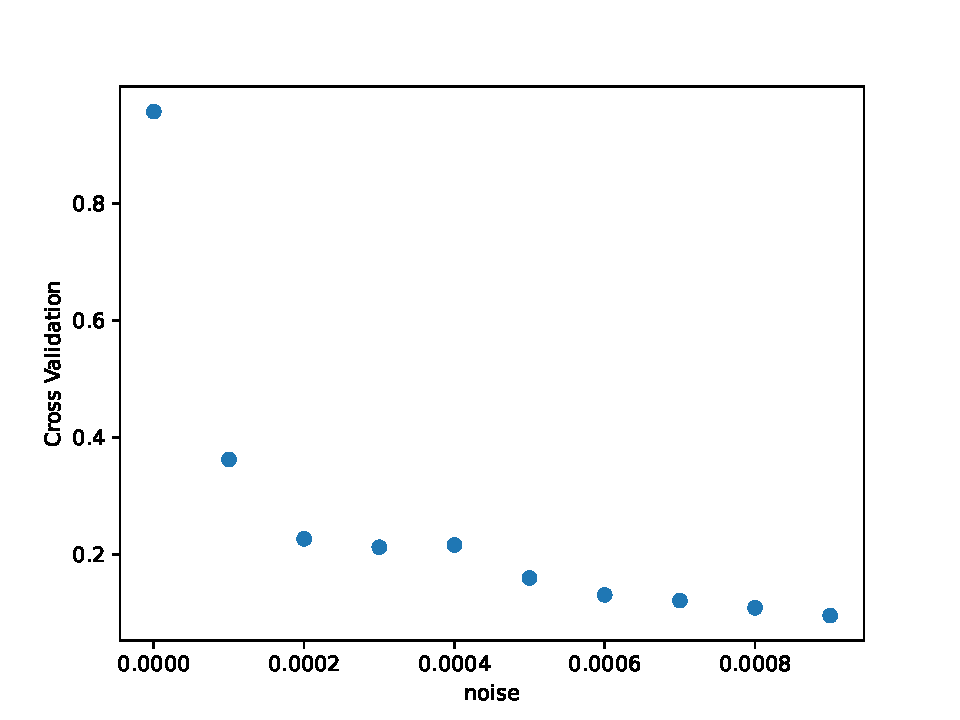
\includegraphics[width=0.7\linewidth]{figures/rrlda_lda_cv_noise.pdf}
    \caption{Cross validation of Reduced Rank LDA under different noise variance.}
    \label{fig:rrlda_lda_cv_noise}
\end{figure}

\begin{figure}
    \centering
    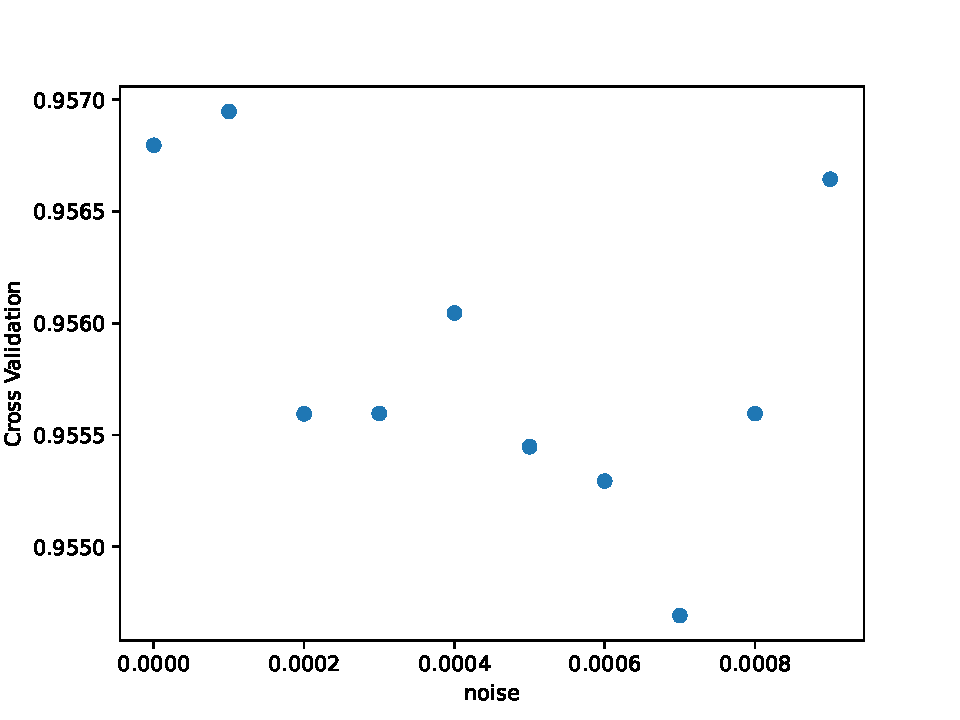
\includegraphics[width=0.7\linewidth]{figures/pca_lda_cv_noise.pdf}
    \caption{Cross validation of PCA under different noise variance.}
    \label{fig:pca_lda_cv_noise}
\end{figure}

\begin{table}
    \centering
    \caption[short]{Cross Validation and AIC Result}
    \label{tab:cv-result}
    \begin{tabular}{c|ccc}
        \hline\hline
        Model & AIC & CV & Accuracy\\ \hline\hline
        Reduced Rank LDA &  & 0.9541 & 0.0560 \\
        PCA + LDA & 0.9649 & 0.9548 & 0.9447 \\
        PCA + SVM-1 & 0.7858 & 0.7790 & 0.7647 \\
        PCA + SVM-2 & 0.0489 & 0.0489 & 0.0378 \\
        PCA + SVM-3 & 0.0489 & 0.0489 & 0.0378 \\
        PCA + MLP-100 & 1.0 & 0.9532 & 0.9251 \\
        PCA + MLP-200 & 1.0 & 0.9551 & 0.9286 \\
        PCA + MLP-300 & 1.0 & 0.9535 & 0.9321 \\
        PCA + MLP-400 & 1.0 & 0.9577 & 0.9349 \\
        \hline\hline
    \end{tabular}
\end{table}